\documentclass[]{scrartcl}

\usepackage{graphicx}
\usepackage{soul}
\usepackage{caption}
\usepackage{amsmath}
\usepackage{amssymb}
\usepackage{amsthm}
\usepackage{subcaption}
\usepackage[utf8]{inputenc}
\usepackage[top=1.5in, bottom=1.5in, left=1in, right=1in]{geometry}
\usepackage{xcolor}
\usepackage{framed}
\usepackage{booktabs}

\makeatletter
\newtheoremstyle{break}
   {\topsep}{\topsep}%
   {\itshape}{}%
   {\bfseries}{}%
   { }
   {\thmname{#1}\thmnumber{\@ifnotempty{#1}{ }\@upn{#2}}%
    \thmnote{ {\bfseries(#3)}}.}% 
\makeatother
\theoremstyle{break}

\newtheorem{definition}{Definition}
\newtheorem{invariant}{Invariant}
\newtheorem{example}{Example}

\newcommand{\mt}[1]{\textnormal{#1}}
\renewcommand{\tt}[1]{\texttt{#1}}
\colorlet{shadecolor}{yellow!60}
\newcommand{\highlight}[1]{\colorbox{yellow!70}{#1}}
\newcommand{\shade}[1]{\begin{shaded}#1\end{shaded}}

\newcommand{\N}{\mathbb{N}}
\newcommand{\Q}{\mathbb{Q}}
\newcommand{\R}{\mathbb{R}}
\newcommand{\B}{\mathbb{B}}
\newcommand{\allQ}[1]{\left[\forall #1 \right]}

\newcommand{\co}{\mathbf{Co}}
\newcommand{\cansend}[2]{#1 \rightarrowtail \{#2\}}
\newcommand{\cantsend}[2]{#1 \stackrel{\times}{\rightarrowtail} \{#2\}}
\newcommand{\canrec}[2]{\{#1\} \rightarrowtail #2}
\newcommand{\cantrec}[2]{\{#1\} \stackrel{\times}{\rightarrowtail} #2}
\newcommand{\rec}[1]{\tt{rec}(#1)}
\newcommand{\ft}[1]{\tt{ft}_{#1}}
\renewcommand{\int}[1]{\tt{int}_{#1}}
\newcommand{\proc}[1]{\tt{proc}_{#1}}
\newcommand{\sends}[3]{#1 \rightarrow [#2] \rightarrow #3}
\newcommand{\sendsm}[4]{#1 \rightarrow [#2 , #3] \rightarrow #4}
\newcommand{\sendsf}[6]{#1\langle #2 \rangle \rightarrow [#3,#4] \rightarrow \langle#5\rangle#6}

\newcommand{\compT}[2]{\tt{Comp}_{#1,#2}}

\DeclareMathOperator{\tint}{int}
\newcommand{\type}[1]{\mathtt{#1}}
\DeclareMathOperator{\cint}{cint}

%opening
\title{{\huge A Proposed Evolutionary Model of Cognition}}
\author{Janos Tapolczai}

\begin{document}

\maketitle

\begin{abstract}

\end{abstract}

\tableofcontents
\newpage

\section{Introduction}

In this document, I will sketch a possible architecture of the human brain and a select few of its subsystems. The descriptions presented are supported by some empirical evidence, but I do not claim that they are straightforward transcriptions of neurological realities. The model is grounded substantially in evolutionary considerations, which provide the backdrop and the plausibility check for the claims presented herein.

Section~\ref{sec:preliminaries} outlines the basic considerations that lead to the model. Section~\ref{sec:globalArchitecture} sketches the proposed model of the mind. Section~\ref{sec:mathematicalModel} presents the mathematical model. In Section~\ref{sec:selectedSubsystems}, we look at three concrete subsystems: sensory perception, counterfactual perception (imagination) and affect.

It should also be understood that everything in this document is, at best, a {\em rough} outline; it may be likened to a hexagon which approximates a circle: though (conjectured to be) basically correct, and useful, it is marred by significant incongruities with the object of its approximation.

\section{Preliminary considerations and justification}\label{sec:preliminaries}

In order to understand how our brain works or could work, we must possess conceptual clarity --- we must conceive of it, not as a product of engineering, but as a historical artefact, and as one which was not produced ``in one step'', but gradually, where each stage of its evolution had to be viable on its own. What, one might ask, is the consequence of such a view?
Most importantly, it allows the distinction between what I will herein call \textsc{efficient} systems and \textsc{clean} systems. Since, at each stage of its evolution, the organism that carried the brain had to be viable, the end product is by definition guaranteed to be ``efficient''. Because of that same fact, however, it is all but guaranteed not to be ``clean'': for one, it was not possible to snap whole new components into the system; it would have also been impossible to combine old components in the elaborate and precise ways in which a human engineer might use parts. Worse, old components were almost certainly not discarded when new and better components came into being. A good exposition of this process in humans can be found in Paul MacLean's seminal work {\em The Triune Brain in Evolution} \cite{maclean1990}.

\begin{figure}[!h]
	\centering
	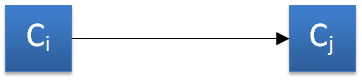
\includegraphics{figs/noNervousSystem.png}
	\caption{Relationship between the components of an organism without a nervous system.}
	\label{fig:noNervousSystem}
\end{figure}
\vspace{-0.18cm}
\paragraph{Origin of nervous systems} The evolution of nervous systems in organisms dates back to the development of primitive electrical signalling in eukaryotes, using calcium action potentials.\footnote{See any textbook on evolutionary biology.} The benefits of such mechanisms were obvious: let us imagine a microscopic organism without any sort of nervous system --- all of its behaviour is hard-coded and mechanical. It can take in nutrients through its cell walls or through an opening; parts of it can contract or expand in response to stimuli like light or pressure; homeostatic conditions can influence its chemistry. Figure~\ref{fig:noNervousSystem} shows this schema: if we enumerate the constituent parts or {\em components} of an organism as $\{C_1,\dots,C_n\}$, the organism's behavior is caused by signals being sent between $C_i$ and $C_j$ (the case $i=j$ is of course possible). Such an organism suffers from two disadvantages: (a) the behaviour is necessarily simple and (b) it is not very adaptable.

Let us now imagine that such an organism develops a bundle of cells which transmit the signals from various parts of its body, modulate them in some way, and then send them to various parts, inducing changes. Schematically, this is shown in Figure~\ref{fig:nervousSystem}, where a function $F$ is interposed between two components. The first such nervous systems were likely little more than signal transformers or magnifiers that expedited communication between parts: with a few neurons, an organism would have had the ability to coordinate movements or rely on sensing parts induce, say, movement.

\begin{figure}
	\centering
	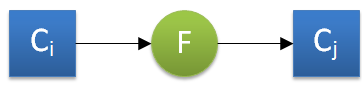
\includegraphics{figs/nervousSystem.png}
	\caption{Relationship between the components of an organism possessing a nervous system. $F$ can be understood as a simple signal transformer or a central coordinating mechanism.}
	\label{fig:nervousSystem}
\end{figure}

The neuron bundles would have been quite malleable in the face of selection pressure: when the environment required it, they could, after several generations, start to compute different or more elaborate functions. For instance, an organism which had had developed in an environment where food was abundant in bright places and which had now found itself in darkness would have benefited from a variety of plausible changes, such as
\begin{itemize}
	\item an inversion of its light-seeking behaviour,
	\item switching off its metabolism in light places to conserve energy,
	\item accelerating its metabolism in dark places to make better use of the food there.
\end{itemize}

Of course, other changes would have also been possible, such as the metabolization of different food sources,\footnote{A current-day example is given by nylon-eating bacteria, which have developed in the last century and which now have an abundant food source and no competition.} but we can see how the aforementioned three could have been effected through changes in a simple nervous system alone. Let us recall the beginning of this section and contrast such a malleable computational mesh with most products of human engineering: one cannot simply take out a piston in a car or replace a cogwheel in a mechanical clock with a differently sized one. Machines are designed to fit together perfectly and their complexity tends to be irreducible. Even programs, which are more open to mutation and which are often evolved in evolutionary algorithms, are easily broken by small changes.

\paragraph{Adaptation of nervous systems}  When discussing how an organism's nervous system can evolve and, in particular, {\em evolve to perform new tasks} and not just variations on old ones, explanations are again constrained by two criteria: (a) the change has to be small, or at least have a small cause\footnote{The effect does not have to be small --- changes in single genes can switch entire components on or off. The MYH16 gene, which is present in non-human primates but has been switched off in humans, is an example. In us, its disabling lead to a drastic reduction in the size of jaw muscles and a corresponding increase in brain size~\cite{carroll2005}.} and (b) each change must be beneficial in the short term.\footnote{Caveats apply: if the selection pressure on a group of organisms isn't too strong, changes which may be sub-optimal but perhaps beneficial at some later point may spread, and non-selective processes like genetic drift can also play a role.}

To illustrate this, we can look at a simple neural network in Figure~\ref{fig:neuralNetwork}, with a marked node $N_x$. Figure~\ref{fig:unlikelyEvolution} shows an unlikely change scenario in which some new component/function is cleanly grafted onto the system. Figure~\ref{fig:likelyEvolution} then shows a much more likely scenario: a mutation causes $N_x$ to be split and the new nodes take over some of its connections. In time, new functions can thus grow into the system, but never in the manner in which, say, an engineer would implement a new feature.

\begin{figure}
	\centering
	\begin{subfigure}[t]{0.45\textwidth}
		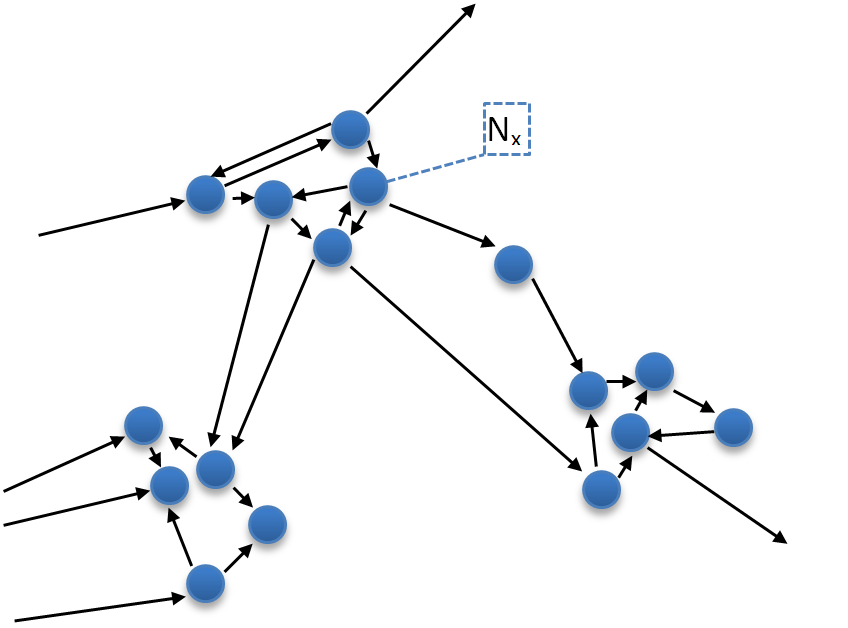
\includegraphics[width=\textwidth]{figs/neuralNetwork.png}
		\caption{A simple neural network.}
		\label{fig:neuralNetwork}
	\end{subfigure}
	\begin{subfigure}[t]{0.45\textwidth}
		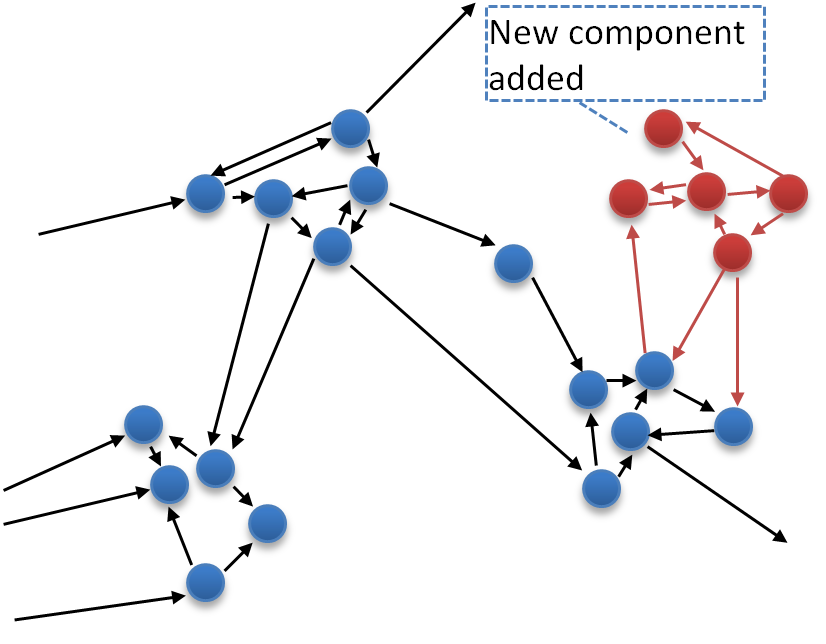
\includegraphics[width=\textwidth]{figs/unlikelyEvolution.png}
		\caption{An unlikely change scenario in which new, discernible components are grafted on from whole cloth.}
		\label{fig:unlikelyEvolution}
	\end{subfigure}
	\begin{subfigure}[t]{0.45\textwidth}
		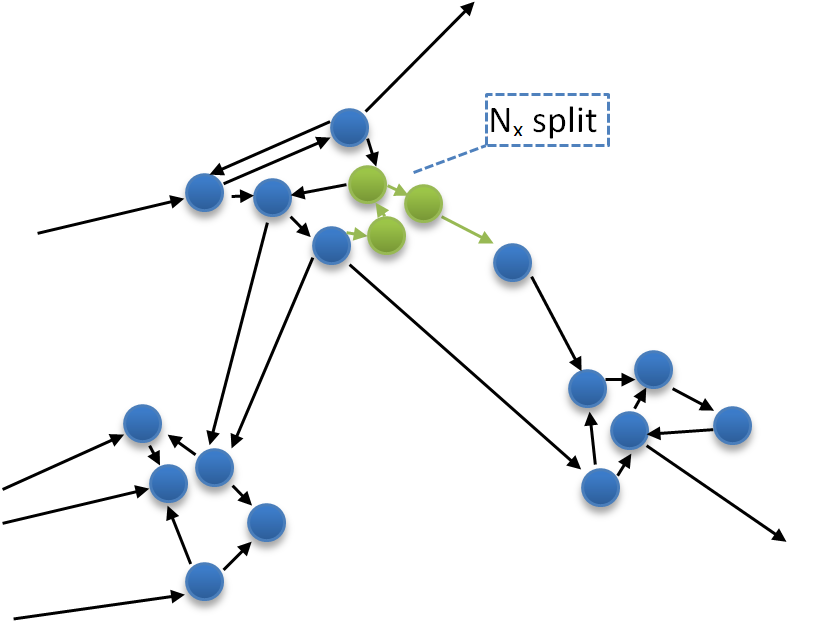
\includegraphics[width=\textwidth]{figs/likelyEvolution.png}
		\caption{A more likely change scenario in which one part is split into three but where the overall shape of the network is not appreciably altered.}
		\label{fig:likelyEvolution}
	\end{subfigure}
\end{figure}

\paragraph{The brain as a collection of functions}

The processes hitherto described are quite uncontroversial and can be found reiterated in any textbook on the evolution of nervous systems. The functional structure and the model of computation used in the brain, however, are not well understood. FMRI and similar brain imagining techniques, while invaluable, give only rough impressions about the neural correlates of certain forms of cognition and do not give fine-grained insight into its structure. As such, the model I shall describe in the following paragraphs is a conjecture. The implication of such an evolutionary viewpoint, I conjecture in this document, is that brain functions don't ``just appear'', but are rather the result of small changes and the recombination of pre-existing parts. This, in turn, informs the plausibility of various possible brain architectures. In becomes unlikely that the brain should be a collection of neatly delineated functions, or that it should have certain coordinating units or universal message formats for communication between components. The reason for this is that administrative mechanism confer little evolutionary benefit on their owen, and do not confer it gradually: the imposition of a central coordinating mechanism on a pre-existing mesh of neurons would necessitate the complete reorganisation of such, and the abandonment of the previous communication channels on favor centralized coordination. The same objections can be raised against a universal or even a local message format. Moreover, such mechanisms require substantial changes in the organism with no obvious or immediate advantage.

Such objections do not contradict the existence of macroscopic structures in the brain, dedicated to certain tasks. The development and adaptation of such remains entirely plausible. They do, however, give insight into the pattern of processing inside such structures, which is often simply regarded as atomic or replicated in computers as if it were a conventional engineering product.

Instead of a rigidly ordered brain with central organisation and large, discrete, and highly complex features like ``sight'' or ``reason'' which function like pluggable black boxes, I propose a decentralized white-box architecture composed of simple parts: first, every component, while perhaps sophisticated, is conceptually simple. Second, communication between different components is not performed in the function-call pattern of computer programs, but rather by one component listening in on the activity of another. Since there is, inherently, no mechanism of function abstraction in neural systems, it stands to reason that the most likely way for new functions to develop is for additional neurons to modulate the activity of others. In such a scheme, a visual perception component doesn't have to know which other components will consume its output (or rather, listen on its activity); changes which affect agent activity in useful ways based on the visual data can occur gradually and, over time, become large enough to count as components in their own right.

\paragraph{Practical abstraction}

While such a white-box model is conceptually useful, a mesh of gradually grown patterns does not lend itself to implementation in a program. Therefore, I will present a simplified model which, while attempting to remain true to the conceptual view, will, pragmatically, contain discrete functions and components. The white-box nature of brain activity will be emulated by a message-passing scheme in which messages model the internal activity of components. Instead of each component blindly acting in some fashion on the activity of another, components will have explicit parsers and interpreters and later, these will be further simplified into localized message formats and tagging, for the sake of easy implementation.

\section{Diagram notation}

In the rest of this document, a number of diagrams appear. These will use the following notation:

\begin{center}
	\begin{tabular}{p{.5\textwidth}@{}p{.4\textwidth}@{}}
		\toprule
		Symbol & Description\\
		\midrule
		
\includegraphics[width=80pt]{figs/legend_proc.png} \dotfill & Processing component\\
		
\includegraphics[width=80pt]{figs/legend_choice.png} \dotfill & Choice\\
		
\includegraphics[width=50pt]{figs/legend_container.png} \dotfill & Data container (Queue, List, etc.)\\
		
\includegraphics[width=50pt]{figs/legend_data.png} \dotfill & Data\\
		
\includegraphics[width=30pt]{figs/legend_generator.png} \dotfill & Stream generator\\
		
\includegraphics[width=50pt]{figs/legend_imaginary.png} \dotfill & Counterfactual (imaginary) data\\
		\bottomrule
	\end{tabular}
\end{center}

\section{Global architecture}\label{sec:globalArchitecture}

We can imagine the components of the mind as white boxes which inform other components by their very functioning --- however, this does not lend itself to easy implementation. Instead, we can emulate this behaviour via a \caps{message space}, from which individual components take their input and into which they put their output. A \caps{component} is then a local processing unit which continuously scans the message space, running messages through its \caps{filter}. If the filter detects a relevant message, it is then passed to the \caps{interpreter}, which parses the message into the needed format and hands it over to the \caps{processor}. The processor, after having finished, puts its output back into the message space for other other components to read. Figure~\ref{fig:global} illustrates this scheme. Note the lack of explicit hierarchical structure and central organising units.

\begin{figure}[!h]
	\centering
	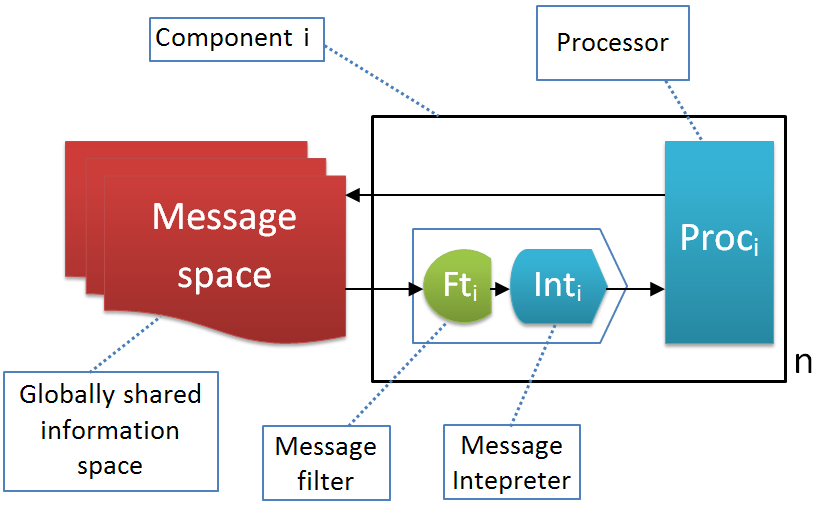
\includegraphics[width=400pt]{figs/global.png}
	\caption{Global neural architecture.}
	\label{fig:global}
\end{figure}

However, as I'll show in the next section, this model is generic enough to accommodate such special-purpose structures. Figure~\ref{fig:global} shows the message-passing scheme, but it also specifies a graph in which the nodes are the components and fixed, while the edges are the accepted messages and are determined by the nodes; through their filters, components control the shape of the graph. By imposing invariants on these filters, we can have the graph take any shape we desire. In particular, we can model the kinds of structures that occur in many other cognitive models and in empirical research: central organisers, sequences of components (``pipelines''), localized messages affecting only a small part of the mind, a component reading its own messages, loops and iterative messages between two or more components et cetera.

\pagebreak

\paragraph{Messages}

We may now ask how such messages between components are structured. Here, I make two empirical claims:
\begin{enumerate}
	\item messages have a priority and
	\item they are effectively unstructured.
\end{enumerate}

\begin{figure}[!h]
	\centering
	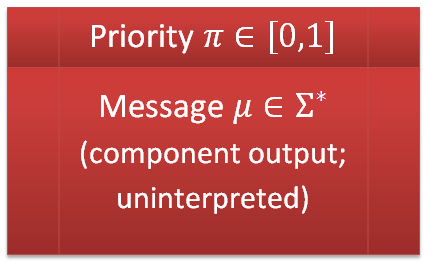
\includegraphics[width=150pt]{figs/message.png}
	\caption{Structure of a neural message.}
	\label{fig:message}
\end{figure}

To the best of my knowledge, the veracity of either has thus far not been determined by neuroscience. For the first, Marvin Minsky's ``The Emotion Machine'' provides some circumstantial evidence \cite[p. 222]{emotionMachine}:

\begin{quote}
	Of course, when one activates two or more Critics or Selectors, this is likely to cause some conflicts, because two different resources might try to turn on a third resource both {\em on} and {\em off}. To deal with this, we could design the system to use various policies like these:
	
	\begin{enumerate}
		\item Choose the resource with the highest priority.
		\item Choose the one that is most strongly aroused.
		\item Choose the one that gives the most specific advice.
		\item Have them all compete in some ``marketplace''.
	\end{enumerate}
\end{quote}

The selection strategies Minsky lists imply that there is some mechanism in the brain to determine the urgency of a signal. While it is possible that higher brain functions like reasoning or affect make an additional, rational evaluation, sensations like intense pain, bright lights, or great sadness can likely be communicated most easily by the appropriate components causing a flood of activity which, by its very intensity, informs other components of the urgency of their messages.

The second claim --- that messages are essentially unstructured --- means that there is no common, agreed-upon format in which they are stored. In addition to the evolutionary implausibility of such a format being created, an unstructured message format is in line with the white-box nature of components: since components merely ``listen in'' on others, and since each components will have its own pattern of activity, a listener would simply have to try and make sense of this activity as best it could. The proposed structure of messages is thus shown in Figure~\ref{fig:message}: every message comprises a priority header, together with an unstructured body which, for our purposes, is simply a string of bits.

\paragraph{Filters} Before a component can respond to a message by another, such a message must be assessed for the presence of relevant information. Conceptually, this happens via a \caps{filter} in each component, which pattern-matches incoming messages and, if a certain threshold is reached, signals relevance and hands the message over the \caps{interpreter} for parsing. Figure~\ref{fig:filter} shows such a filter: it is composed of a directed graph of nodes, and a node is activated if it detects some specific content in the message. Nodes, in turn, are connected via edges of strength $\in [0,1]$. When a node is activated, it sends a charge proportional to the strength of its link to its neighbours, contributing to their activation as well. Some nodes are marked as {\em output nodes}; if enough such output nodes become activated, the message is deemed to be sufficiently relevant. This model of filters is inspired by the {\em spiking neural P Systems} of Georghe Pa\u{u}n et al. (\cite[p. 337]{membraneComputing} and \cite{spikingNeural}), in which charges sent along directed graphs of neurons are used to compute functions.

\begin{figure}[!h]
	\centering
	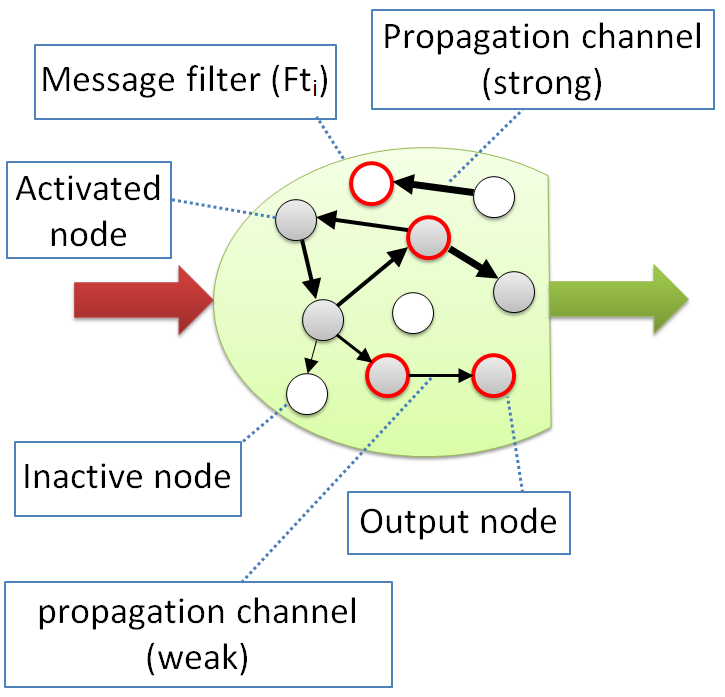
\includegraphics[width=215pt]{figs/filter.png}
	\caption{A pattern-matching filter for a component $C_i$.}
	\label{fig:filter}
\end{figure}

\section{Mathematical model}\label{sec:mathematicalModel}

We now create a mathematical model for the description of the architecture of Section~\ref{sec:globalArchitecture}. This model will be split into two parts: the structural and the operational semantics. The structural semantics encode the static properties of neural systems, whereas the operational semantics describe the behaviour of such a system at runtime.

\subsection{Preliminaries}\label{sec:mathematicalPreliminaries}

Since the mathematical model is built with implementation in mind, I will use some basic type theory in the coming sections. In this section the relevant notions will be introduced, without assuming any prior knowledge. 

\begin{definition}[Syntax: Type]\label{def:type}
For our purposes, types are defined inductively thus:
	\begin{enumerate}
		\item[Basic type.] The sets $\N$, $\Q$, $\R$, $\B$ are types.
		\item[Sum type.] If $\type{T_1},\type{T_2}$ are types, the sum type $\type{T_1 + T_2}$, is a type. 
		\item[Product type.] If $\type{s}$ is a string and $\type{T_1},\dots,\type{T_n}$ are types, the product type $\type{s}\ \type{T_1} \dots \type{T_n}$, is a type. A special case is the {\em anonymous product type} (tuple), where $s=``\langle\rangle"$. There, we just write $\langle\type{T_1},\dots,T_n \rangle$.
		\item[Full application.] If $\type{T_1},\dots,\type{T_n}$ are types and $\allQ{x_1,\dots,x_n} \type{C}$ is a type constructor (see next definition), then $\mathtt{C\\type{T_1} \dots \type{T_n}}$, is a type.
	\end{enumerate}
\end{definition}

\begin{definition}[Semantics: Type]\label{def:typeSem}
Semantically, every type $T$ is simply a set of values. We denote this set with the interpretation function $\tint(T)$.
	\begin{enumerate}
		\item[Basic type.] $\tint(\B) = \{ \tt{false}, \tt{true} \}$. $\N, \Q, \R$ are interpreted as the natural, rational, and real numbers, respectively.
		\item[Sum type.] If $\type{T_1}, \type{T_2}$ are types, then $\tint(\type{T_1 + T_2}) = \tint(\type{T_1}) \cup \tint(\type{T_2})$.
		\item[Product type.] If $\type{T_1},\dots,\type{T_n}$ are types, then $\tint(\type{s}\ \type{T_1} \dots \type{T_n}) = \{s\} \times \tint(\type{T_1}) \times \dots \times \tint(\type{T_n})$.
		\item[Full application.] If $\type{T_1},\dots,\type{T_n}$ are types and $\allQ{x_1,\dots,x_n} \type{C}$ is a type constructor, then $\tint(\type{C}\ \type{T_1} \dots \type{T_n}) = \bigcup\limits_{v_1 \in\ \tint(T_1)} \cdots \bigcup\limits_{v_n \in\ \tint(T_n)} \bigcup\limits_{C' \in\ \cint(C)} C'[x_1\backslash v_1,\dots, x_n\backslash v_n]$.
	\end{enumerate}
\end{definition}

We now define type constructors which quantify over types:

\begin{definition}[Syntax: Type constructor]\label{def:typeCon}\
	\begin{enumerate}
		\item[Base case.] Every type $\type{T}$ is a type constructor.
		\item[Abstraction.] If $\type{C}$ is a type constructor and $\type{T}$ is a type, $\allQ{x} \type{C}[\type{T}\backslash x]$ is a type constructor.
		\item[Sum types.] If $\type{C_1}\dots,\type{C_n}$ are type constructors with $\type{C_i} = \allQ{x^i_1\dots,x^i_n} \type{T_i}$ ($1 \leq i \leq n$), then\\ $\allQ{x_1,\dots,x_n} (\type{C_1} + \dots + \type{C_n})$ is a type constructor.
		\item[Partial application.] If $\type{T_1},\dots,\type{T_i}$ ($i < n$) are types and $\allQ{x_1,\dots,x_n} \type{T}$ is a type constructor,\\ then $\allQ{x_{i+1},\dots,x_n} \type{T}[x_1\backslash \type{T_1},\dots,x_i\backslash \type{T_i}]$ is a type constructor.
	\end{enumerate}
\end{definition}

\begin{definition}[Semantics: Type constructor]\label{def:typeConSem}
Type constructors have a partial interpretation function $\cint$, defined thus: if $\type{C}$ is a type constructor containing exactly the types $\type{T_1},\dots,\type{T_n}$, then $\cint(\type{C}) = \bigcup\limits_{v_1 \in\ \tint(T_1)} \cdots \bigcup\limits_{v_n \in\ \tint(T_n)} \type{C}[T_1\backslash v_1,\dots,T_n\backslash v_n]$.
\end{definition}

Intuitively, sum types are simply unions, product types are named cartesian products, and full applications are instantiations of type constructors with all possible values. Type constructors themselves are just generic types.

Henceforth, by convention, we will write type variables in lower-case and concrete types in upper-case, omitting the explicit $\forall$-blocks. That is, a type like $\allQ{x,y,z} \type{C\ x\ (\N + T_1)\ y\ z}$ will simply be written as $\type{C\ x\ (\N + T_1)\ y\ z}$ and it will be clear that $\type{x}, \type{y}, \type{z}$ are type variables, while $\N, \type{T_1}$ are concrete types.\\

A special kind of type constructor is the function arrow ($\rightarrow$) which induces the function type:

\begin{example}[Function arrow]
	$\rightarrow \type{s}\ \type{t}$ is the type constructor for unary functions from $\type{s}$ to $\type{t}$. We also write this infix as $\type{s} \rightarrow \type{t}$. Functions with multiple arguments, mapping $\type{t_1},\dots,\type{t_{n-1}}$ to $\type{t_n}$, are modelled via nested function arrows:
	
	$$
		\type{t_1} \rightarrow (\type{t_2} \rightarrow \dots \rightarrow (\type{t_{n-1}} \rightarrow \type{t_n})\cdots)
	$$
\end{example}

\noindent
We can combine type constructors, sum types, and product types into {\em algebraic data types} (ADTs).

\begin{definition}[Algebraic data type (ADT)]\label{def:ADT}
Let $\type{s}$ be a string and $\type{C_1},\dots,\type{C_n}$ be type constructors s.t. $\type{C_i} = \allQ{x_1,\dots,x_n} \type{T_i}$ and $\type{T_i}$ is a named product type with type variables ($1 \leq i \leq n$). Then $\allQ{x_1,\dots,x_n} (\type{T_i} + \dots + \type{T_n})$ is an ADT. If we want to give a name to an ADT, we write it as $\type{s\ x_1 \dots x_n = T_i + \dots + T_n}$.
\end{definition}

Since an ADT is merely the sum of product types, it is itself a type constructor. If it has no type variables, it is also a type. Next, we define three ADTs which we will use in the next section: \tt{Maybe}, \tt{Either}, and \tt{List}.

\begin{example}[Maybe, Either, List]
	$$
		\begin{array}{l l}
			\type{Maybe\ t} & = \type{Nothing + Just\ t}\\
			\type{Either\ l\ r} & = \type{Left\ l + Right\ r}\\
			\type{[]\ a} & = \type{[] + (a : [a])}\\
		\end{array}
	$$ 
	
	$\mathtt{Maybe}$ represents an optional value, which may or may not be present. $\mathtt{Either}$ represents a choice between two values, of which either the left or the right one is present, but not both. $\type{[a]}$ denotes a list of values of type $\type{a}$.
\end{example}

Definitions~\ref{def:type}--\ref{def:ADT} specify a fragment of System F$_\omega$,\footnote{Specifically, the decidable fragment of System F$_\omega$ without higher kinds and only prenex-polymorphism. That is, type constructors can only take types as arguments and are of the form $\allQ{x_1,\dots,x_n} \type{C}$ for quantifier-free $\type{C}$. This is also called the Hindley-Milner type system. For details, see Barendregt's paper \cite{barendregt91}.} which is used to type expressions in the lambda calculus. Although System F is strictly more powerful, our definitions are enough to provide a description language for the data types and functions in the rest of this work.


\subsection{Neural systems}\label{sec:mathematicalNeuralSystem}

\begin{definition}[Neural component]
	Let $I$ be an index set and let $\type{T}$ be any type. Then, a neural component $C$ with a name from $I$ and message type $\type{T}$ is a four-tuple
	$$
		\langle i, \tt{ft}, \tt{int}, \tt{proc} \rangle
	$$
	where
	\begin{enumerate}
		\item $i$ is an element of $I$ and is called the {\em name} of $C$,
		\item $\tt{ft}$ is a function $\type{T \rightarrow \B}$, called the {\em filter} of $C$,
		\item $\tt{int}$ is a function $\type{T} \rightarrow \type{Maybe\ T}$, called the {\em interpreter} of $C$, and
		\item $\tt{proc}$ is function $\type{T} \rightarrow \type{T}$, called the {\em processor} of $C$.
	\end{enumerate}
	
	Formally, the type of $C$ is $\tt{Comp}_{\type{T},I}$. As a shorthand, we denote the name, filter, interpreter and processor of a given component $C$ as $\tt{name}_C$, $\tt{ft}_C$, $\tt{int}_C$, $\tt{proc}_C$, respectively.
\end{definition}

\noindent
A set of neural components, together with a set of messages, induces a {\em neural system}:

\begin{definition}[Neural system]
	Let $T$ be any type and let $I$ be an index set. Then, a neural system with message type $T$ and component names from $I$ is a tuple
	$$
		\langle \textbf{Co}, \textbf{Me} \rangle
	$$
	where
	\begin{itemize}
		\item $\textbf{Co}$ is a set of neural components (with message type $T$ and names from $I$) and
		\item $\textbf{Me}$ is a set of elements of type $T$, called the {\em set of messages}.
	\end{itemize}
\end{definition}

\subsection{Sending and receiving messages}\label{sec:notation}

We now give a notation for the sending and receiving of messages in a system. Here, we distinguish two aspects: first, the structural, which describes how messages {\em can} travel in a system and the operational, which describes how they {\em do} travel in some given scenario.

\subsubsection{Structural notation}

The elements of a component statically determine which messages it can receive and send. Based on the behaviour of the filter, interpreter and processor of a component, we can express a number of properties.

\begin{definition}[Message reception]
	Let $C$ be a component and $m$ be a message. $C$ can receive $m$ if and only if $\ft{C}(m) = \tt{true}$ and $\int{C} = \tt{Just } m'$ for some $m'$.
	When $C$ can receive all messages in $\{m_1,\dots,m_n\}$, we write:
	$$
		\canrec{m_1,\dots,m_n}{C}.
	$$
	
	We denote the opposite statement --- that $C$ cannot receive any message in $\{m_1,\dots,m_n\}$ --- by:
	
	$$
		\cantrec{m_1,\dots,m_n}{C}.
	$$
\end{definition}

\begin{definition}[Message sending]
	Let $C$ be a component and $m, m_1,\dots,m_n$ be messages. $C$ can send out a message $m$ if and only if there exists a message $m_{\mt{in}}$ s.t. $\proc{C}(m_{\mt{in}}) = m$.
	When $C$ can send all messages in $\{m_1,\dots,m_n\}$, we write:
	
	$$
		\cansend{C}{m_1,\dots,m_n}.
	$$
	
	The opposite statement --- that $C$ cannot send any message in $\{m_1,\dots,m_n\}$ --- is again denoted by:
	$$
		\cantsend{m_1,\dots,m_n}{C}.
	$$
\end{definition}

\begin{definition}[Receiving set]
	The set of components which can receive a message $m$ is denoted by
	
	$$
		\rec{m} \equiv \{C \in \co\ |\ \canrec{m}{C} \}.
	$$
	
	\tt{rec} can also be overloaded to refer to the set of components which can receive and interpret at least some message of a component $C$:
	
$$
	\rec{C} \equiv \{C_i \in \co\ |\ \exists m:\ \cansend{C}{m} \wedge \canrec{m}{C_i} \}.
$$
\end{definition}


\subsubsection{Operational notation}

Whereas the structural notation pertained to the static properties of a neural system, the operational notation describes {\em traces}: lists of sent and received messages, and the changes they induced in the system.

\begin{definition}[Message action]
	When a component $C_i$ outputs a message $m_{out}$ that another component $C_j$ receives and interprets as message $m_{in}$, we write
	
	$$
		C_i \rightarrow [m_{out}, m_{in}] \rightarrow C_j.
	$$
	
	We refer to this as {\em message action}. If it's clear that the message $m$ doesn't change, we just write
	
	$$
		C_i \rightarrow [m] \rightarrow C_j.
	$$
\end{definition}

\begin{definition}[Trace]
	Traces are defined inductively thus:
		\begin{enumerate}
			\item Every message action is a trace.
			\item If $T_1$ and $T_2$ are traces, $T_1;T_2$ is a trace.
		\end{enumerate}
		
	$;$ denotes sequential execution and is associative. Thus, the semantics of a trace $T_1;T_2;\dots;T_n$ are that $T_1$ is executed first, followed by $T_2$, and so forth, until $T_n$ is reached and the execution ends.
	For readability, $T_1;\dots;T_n$ will sometimes be written line-by-line as
	$$
		\begin{array}{l}
		T_1\\
		\vdots\\
		T_n
		\end{array}
	$$
\end{definition}

\begin{definition}[Component mutation]
	Let $f_1,f_2,\dots$ be functions $\compT{T}{I} \rightarrow \compT{T}{I}$ which preserve the names of components, $m,m'$ be messages of type $T$, and let $C$ be a component of type $\compT{T}{I}$. When $C$ is changed into $f_n \circ \dots \circ f_1 (C)$ by a message $m$ it receives, or changed into $f_n \circ \dots \circ f_1 (C)$ by a message $m'$ it sends, we write, respectively:
	$$
		\begin{array}{c}
			\dots \rightarrow [m] \rightarrow \langle f_1,\dots,f_n \rangle C\\
			C\langle f_1,\dots,f_n \rangle \rightarrow [m'] \rightarrow \dots
		\end{array}
	$$
	
	\noindent
	If no change occurs, that is, if
	$$
		\begin{array}{r l}
			C\langle\rangle \rightarrow [m] \rightarrow \dots & \mt{or}\\
			\dots \rightarrow [m] \rightarrow \langle\rangle C
		\end{array}
	$$
	
	\noindent
	we omit the angle brackets.
	The semantics are as follows: after by sending or receiving a message, $\co$ is replaced by $(\co - \{C\}) \cup \{f_n \circ \dots \circ f_1 (C) \}$.
\end{definition}

\begin{definition}[Plastic and non-plastic neural systems]
	If, for all messages $m$ and components $C, C'$ in a neural system, the following holds:
	$$
		C\langle\rangle \rightarrow [m] \rightarrow \langle\rangle C'
	$$
	
	\noindent
	we call the system non-plastic. Otherwise, we call it plastic.
\end{definition}


This definition intends to roughly convey the notion of neuroplasticity, as used in neuroscience: areas in the brain are changed over time through specific patterns of activity. Here, such change is modelled by the execution of functions and the replacement of $C$ in the system by $f_n \circ \dots \circ f_1 (C)$.

\subsection{Invariants}

Such a model does not necessitate the existence of special structures, such as central organizers or sequences of components, one activated after another,\footnote{An example of such a sequence is found in \cite{DBLP:journals/nn/SanderGS05} where the authors model the emotion process as a four-step pipeline of relevance, implication, coping and normative significance.} but it does not preclude them either. In fact, we can enforce certain features via first-order invariants. For example, a central organizing units for the components $C_1,\dots,C_n$ can be emulated by a component $C_{co}$ which accepts messages and transforms them into an appropriate format for the some other components.

\begin{invariant}[Central organiser]
$$
	\begin{array}{l}
	 [\forall i \in \{1\dots,n\}] [\forall m]:\\
	 \quad \quad \left(\cansend{C_i}{m} \Rightarrow \rec{m} = \{C_{co}\}\right) \wedge \left( \left( \proc{C_{co}} \circ \int{C_{co}}(m)  \right) \in \bigcup\limits_{1 \leq j \leq n} \rec{C_j} \right)
	\end{array}
$$
\end{invariant}

Figure~\ref{fig:centralOrganizer} depicts such an organizer. Similarly, sequences can be created by components $C_{1},\dots,C_{n}$, where each components reads the message of the last one.

\begin{invariant}[Sequence]
$$
	[\forall i \in \{2\dots,n\}]:\ \rec{C_{i-1}} = \{C_i\}
$$
\end{invariant}

\begin{figure}
	\centering
	\begin{subfigure}[t]{0.45\textwidth}
		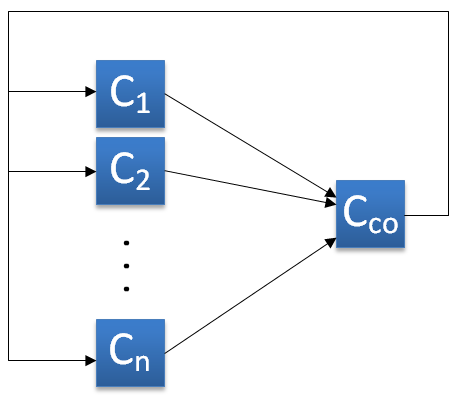
\includegraphics[width=\textwidth]{figs/c_co.png}
		\caption{Components communicating via a central organising mechanism.}
		\label{fig:centralOrganizer}
	\end{subfigure}
	\begin{subfigure}[t]{0.45\textwidth}
		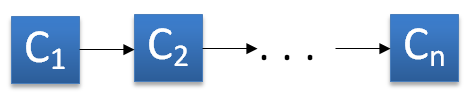
\includegraphics[width=\textwidth]{figs/c_sequence.png}
		\caption{A sequence of components.}
		\label{fig:c_sequence}
	\end{subfigure}
\end{figure}

\section{Selected subsystems}\label{sec:selectedSubsystems}

The global architecture now specified, we will introduce three related subsystems and fit them into this global framework: sensory perception --- the processing of raw sensory input into an format intelligible to other brain components ---, counterfactual perception --- the imagination, which mimics the output of the senses ---, and affect --- broadly speaking, the emotional component of cognition.

\subsection{Sensory perception}\label{sec:sensoryPerception}

The model presented herein is inspired by Marvin Minsky's ``The Emotion Machine''. Therein, Minsky proposes a layered mental structure where each successive layer operates on more and more abstract representations of the world, starting with primitive sensations and proceeding all the way to self-conscious reflection and rational planning. Figure~\ref{fig:brainLayers} shows such a layered structure.

 \begin{figure}[!h]
 	\centering
 	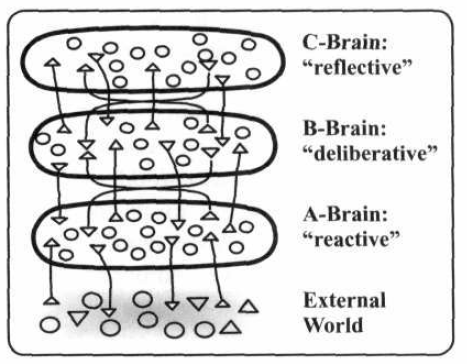
\includegraphics[width=300pt]{figs/emotionMachine_brainLayers.png}
 	\caption{Layered perception of the world, from \cite[p. 100]{emotionMachine}.}
 	\label{fig:brainLayers}
 \end{figure}
 
 \newpage
 
The diagram is explained thus \cite[p. 100]{emotionMachine}:

\begin{quote}
	Now suppose that your A-Brain gets some signals from the external world (via such organs as eyes, ears, nose, and skin) --- and that it also can react to these by sending signals that make your muscles move. By itself, the A-Brain is a separate animal that only reacts to external events but has no sense of what they might mean. For example, when the fingertips of two lovers come into intimate physical contact, {\em the resulting sensations, by themselves, have no particular implications}. For there is no significance in those signals themselves: their meanings to those lovers {\em lie in how they prepresent and process them in the higher levels of their minds.}
\end{quote}

If we apply this to the architecture of Section~\ref{fig:global}, we can devise a system in which each sense $S$ has an associated component $C_S$ which does two things:
\begin{enumerate}
	\item Consume the raw sensory information delivered by various organs and output processed input for higher brain functions;
	\item as a side a effect of this processing, cause  instinctive, low-level reactions in the body, such as pulling away from pain or jumping at a sudden fright.
\end{enumerate}

In Figure~\ref{fig:sensoryPerception}, a slice of just such a system is shown for visual, auditory, olfactory/gustatory and tactile sensation. The produced data can be of two kinds: one is more abstract than the input and facilitates deliberative action, and the other contains instructions for instinctive behaviour for the body.

\begin{figure}[!h]
	\centering
	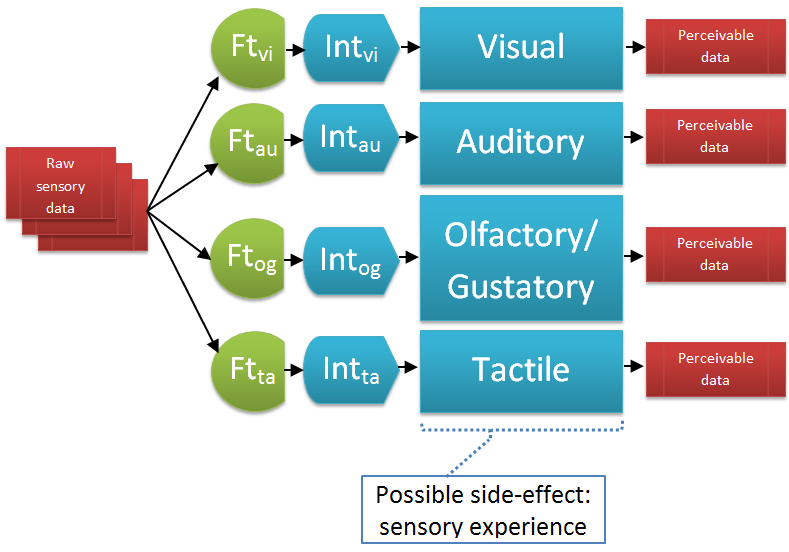
\includegraphics[width=325pt]{figs/sensoryPerception.png}
	\caption{Partial structure of sensory perception - raw sensory data is processed and made available to higher functions such as the affective subsystem. The comment ``Possible side-effect: sensory experience'' signifies the fact that conscious and sub-conscious sensory experiences might occur as a side-effect of this processing. However, it is currently unknown to neuroscience whether this is indeed the case.}
	\label{fig:sensoryPerception}
\end{figure}


\subsection{Counterfactual perception and planning}\label{sec:worldSimulation}

Broadly speaking, counterfactual perception can be described as ``imagination'', and is closely related to sensory perception and world simulation. In examining the system, we might broadly classify its processes into three categories:

\begin{enumerate}
	\item Counterfactual perception --- imagining sights, sounds, etc. Such experiences have much in common with those caused by our sensory organs, yet are marked not as real. In particular, imagined experiences evoke only parts of the conscious experience that accompanies real perceptions. Research by Berthoz and Lotze et al. suggests that (a) the brain indeed uses similar circuitry for real and imagined experiences and that (b) imagined experiences are prevented from being confused with real ones via inhibitory signals. Lotze et al. write \cite{lotze1999}:
	\begin{quote}
		The results of cortical activity support the hypothesis that motor imagery and motor performance possess similar neural substrates. The differential activation in the cerebellum during EM and IM is in accordance with the assumption that the posterior cerebellum is involved in the inhibition of movement execution during imagination.
	\end{quote}
	
	From the abstract of Berthoz's paper \cite{8713551}:
	
	\begin{quotation}
		(...) experimental evidence suggesting that the brain can use the same mechanisms for the imagination and the execution of movement. In particular the fact that adaptation of the vestibulo-ocular reflex can be obtained by pure mental effort and not solely by conflicting visual and vestibular cues has been suggestive of the fact that the brain could internally simulate conflicts and use the same adaptive mechanisms used when actual sensory cues were in conflict.
	\end{quotation}
	
	\item World simulation --- the imagination of future states. Simulating worlds goes beyond the imagination of sensory experiences; it involves constructing models of worlds and simulating their behaviour. The details of this process are unknown, but we can assert that it is capable of a number of things:
	\begin{enumerate}
		\item construction of non-physical worlds, such as mathematical models,
		\item extrapolation into the future and the past
		\item simulation of the minds itself and other agents.
	\end{enumerate}
	
	
	\item Executive planning --- humans can plan both both in immediate and concrete terms (such as body movement) and in the abstract. It is likely that different circuitry is used for movement planning and for planning involving abstract reasoning, in both cases it is necessary that the brain simulate the world in some way. The simulation of the consequences of body movement is likely older than humanity and distinct from the kind of world simulation described above, but both share their function: the agent proposes as series of actions to take, inserts them into some mental world and judges the utility of those actions based on the predicted consequences.
\end{enumerate}

Needless to say, that this process in all its subtleties is immensely complex and thus I simply endeavour to sketch its possible structure only in extremely rough outlines. This sketch is shown in Figures~\ref{fig:imagination},  \ref{fig:planner}, and \ref{fig:worldSimulatorPlannerInteraction}: the world simulation is an ordinary component with a filter and interpreter which outputs, for simplicity's sake, messages marked as counterfactual. We can imagine such messages to be very much like ordinary sensory ones, with the exceptions that they have no accompanying sensation and, more importantly, that we are aware of their non-reality. The planning component receives instructions about desirable states and outputs hypothetical actions which the world simulator incorporates. The world simulator's output is in turn read by the planner, which then abandons the plan or decides to pursue it further.

\begin{figure}
	\centering
	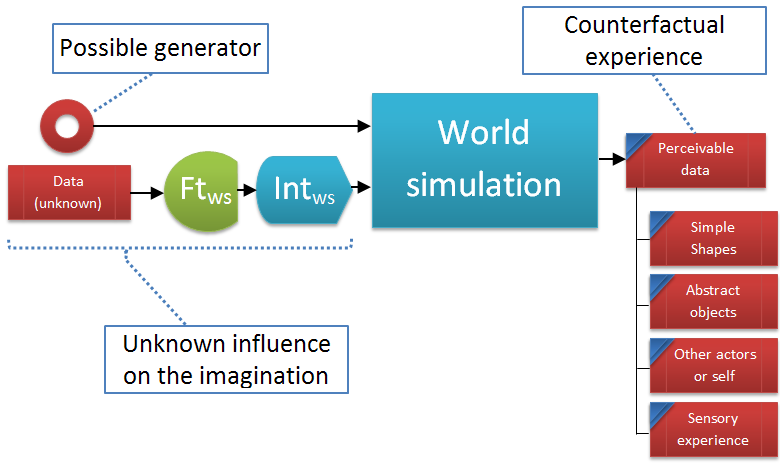
\includegraphics[width=\textwidth]{figs/imagination.png}
	\caption{Structure of of counterfactual perception \& world simulation: messages emulating the output of sensory perception are generated, but are marked as counterfactual by unknown means.}
	\label{fig:imagination}
\end{figure}

\begin{figure}
	\centering
	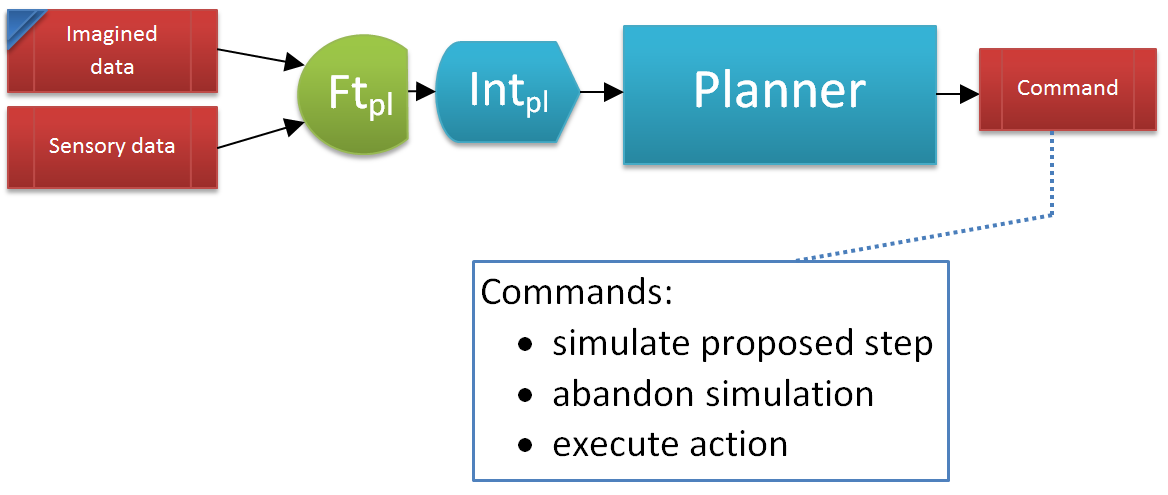
\includegraphics[width=\textwidth]{figs/planner.png}
	\caption{Planner with two kinds of inputs: (1) real sensory data and (2) counterfactual data which comes from world simulation. On the basis of these inputs, possible steps are developed and sent out as commands.}
	\label{fig:planner}
\end{figure}

The planner, minimally, has to perform two functions --- first, it has to judge the desirability of various world states and second, it has to be able to devise possible steps for the agent based on some strategy. If these two functions and some desired goal(s) are given, the planner can do its work by issuing the following commands, as shown in Figure~\ref{fig:planner}:
\begin{enumerate}
	\item If some goals are not yet reached but appear possible, devise possible steps to take and have the world simulator predict their outcomes.
	\item If the goals appear impossible the necessary steps prohibitively undesirable, command the world simulator to cease its activity.
	\item If earlier proposed steps turn out to fulfil some goal, contact the agent's executive component.
\end{enumerate}

\begin{figure}
	\centering
	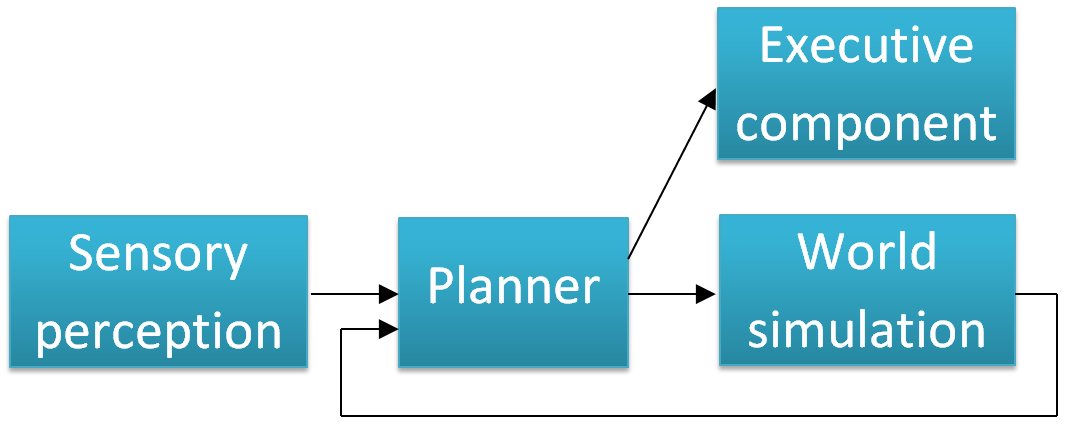
\includegraphics[width=\textwidth]{figs/worldSimulatorPlannerInteraction.png}
	\caption{Interaction between world simulator and planner: the planner devises possible steps and feeds them into the world simulator, which, in turn, tries to calculate their effects. The results are fed back to the planner.}
	\label{fig:worldSimulatorPlannerInteraction}
\end{figure}

\subsubsection{World simulation as rationality}
The way in which I just described the interaction between the world simulator and the planner suggests that they function as a pair of guesser and checker: the planner generates ideas on what to do and the world simulation tests their viability in some setting. Indeed, we can model rational thinking as embedded in the world simulator, especially if we make use of a plastic neural system. The proposed steps of the planner might be quite chaotic and irrational, but when given to the world simulator, it recognises them as such and returns a failure signal to the planner, causing it to abandon ``bad'' paths of cognition. A plastic planner can learn from the consistent failure of certain kinds of steps and, in time, propose them less and less often. Observed as a whole, this system of planner and simulator appears to simply deliver good plans by intuition, even though, in isolation, neither part is very clever.\footnote{I do not wish to idealize rationality too much; world simulation is only partly rational and, given faulty information about the world, will err considerably and in documented ways. Similarly, it is certainly possible for the planner to derange the world simulator by evaluating certain states as so desirable/undesirable that it will pursue even scenarios which the world simulator reports as highly unlikely.}

\paragraph{Model.} In a simplified way, we can model the process of logical deduction in a formal system $F = (A, R)$, where $A$ is a recursive set of axioms and $R$ is a recursive set of production rules of the form $(r_{\mt{from}}, r_{\mt{to}})$ s.t. $r_{\mt{from}} \rightarrow r_{\mt{to}}$ is a valid production in the system. Let
	\begin{enumerate}
		\item $W$ be a world simulator for the world of propositions $\mathcal{P}$ in $(A,R)$,
		\item $P$ a planner,
		\item $St = \{s_1,\dots,s_p\}$ a set of messages about steps to take,
		\item $Cat = \{K_1,\dots,K_q\}$ a list of message categories,
		\item $\tt{cur}$ the current state of the world simulator,
		\item $\tt{ins}\backslash 2$, $\tt{del}\backslash 1$ functions for inserting or deleting a state change into the world simulator or the planner,
		\item $t(i)$ and $b(i)$ functions which increase or decrease the likelihood of sending a message belonging to category $K_i$ and 
		\item $\bot_{i}, \top_{i}$ the failure and success signals of a message belonging to the category $K_i$.
	\end{enumerate}
	
One step of the interaction between $W$ and $P$, in a scenario where $P$ proposes steps $s_{i_1},\dots,s_{i_n}$, can then be modelled with two traces $T_{\mt{guess}}$ and $T_{\mt{check}}$:

$$
	\begin{array}{l l l}
		T_{\mt{guess}}(\tt{step}) & \equiv & \sendsf{P}{\tt{ins}(\tt{cur}, \tt{step})}{\tt{step}}{\tt{step}}{\tt{ins}(\tt{cur}, \tt{step})}{W}\\
		\\
		T_{\mt{check}}(\tt{step}) & \equiv &
		\forall K_i \in Cat: K_i(\tt{step}) \Rightarrow\\
		
		& & \hspace{1cm} \mt{if } \exists (cur, s_j) \in R\ \mt{ then } \
					\sendsf{W}{}{\top_i}{\top_i}{t(i)}{P}\\
		& & \hspace{1cm} \mt{else }\ \sendsf{W}{\tt{del}(\tt{step})}{\bot_i}{\bot_i}{\tt{del}(\tt{step}), b(i)}{P}\\
	\end{array}
$$

\medskip

Axioms can be selected by executing $T_{\mt{guess}}(\tt{ax})$ for all $\tt{ax} \in A$. We can then perform deduction via $T_{\mt{guess}};T_{\mt{check}}$, for a probabilistically selected $\tt{step} \in St$.

Intuitively, $T_{\mt{guess}}$ guesses a step to take. It does so but inserting it into the planner's world-state via $\tt{ins}$ and then sending a message to the world simulator, which also inserts it into its world state. $T_{\mt{check}}$ then checks whether the change from $\tt{cur}$ to $\tt{step}$ was legitimate. If so, it determines to which category $\tt{step}$ belongs and sends the $\top$-signal for that category back to the planner. Otherwise, it sends the corresponding $\bot$-signal. The purpose of this is to make it more or less likely, respectively, that the planner should choose the same category of step in the future. The categories, we can imagine, could be things like ``modus ponens'', ``associative reasoning'', ``appeal to consequences'' and so forth.

If we repeat this interaction (with different proposed steps $s_1,\dots,s_p$ in each iteration), we get an algorithm for logical deduction  --- that is, since $A$ and $R$ are recursive, the system will recursively enumerate all valid logical formulas, provided that we pursue each path and that the probability of selecting any valid step is $> 0$. In addition, we could add a goal function $g$ to $P$ s.t. it would accept certain states and stop. Thereby, $P$ and $W$ could be used to prove logical propositions.

\subsection{Affect}\label{sec:affect}

When discussing human affect, one can mean various things: the causation of emotion, its internal mechanisms, the expression of emotion, social communication of emotions, etc. In this document, we restrict our attention just to the internal mechanisms --- that is, to the means by which emotions are evoked in an agent and how they shape its thinking.

Furthermore, the issue will only be the causative mechanism itself; taxonomy and hierarchy of emotions are deferred to future versions of this document.

The model presented herein is adapted from Gadanho and Hallam \cite{DBLP:journals/adb/GadanhoH01}, who employed it in the context of robot learning. They constructed a system of \caps{feelings} and \caps{sensations} $\mathcal{F}$, \caps{emotions} $\mathcal{E}$, and a hormone storage $H$.

\begin{figure}[!h]
	\centering
	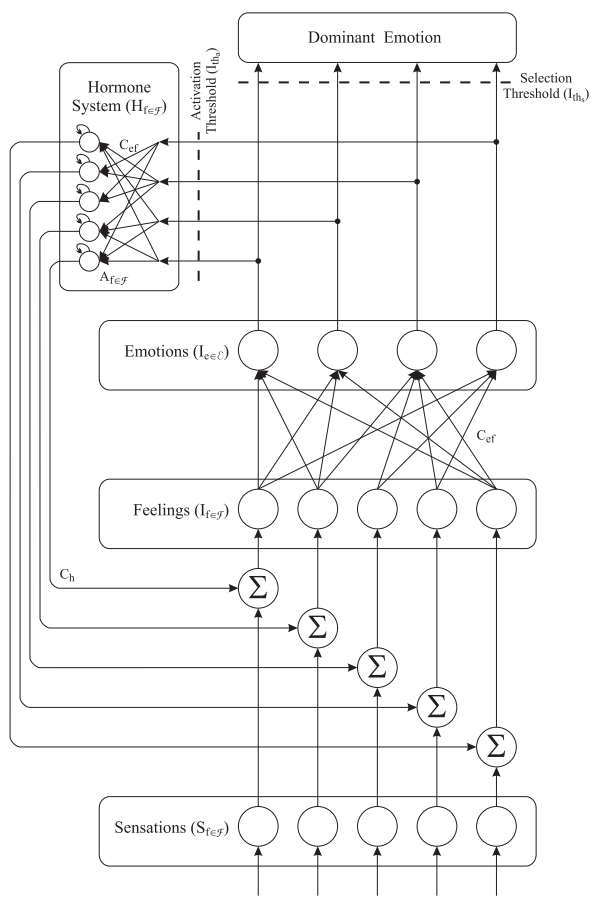
\includegraphics[width=200pt]{figs/gadanhoModel.png}
	\caption{Emotional model of Gadanho and Hallam \cite[p. 46]{DBLP:journals/adb/GadanhoH01}.}
	\label{fig:gadanhoModel}
\end{figure}

Figure~\ref{fig:gadanhoModel} shows this model: \caps{sensations} enter the system and are connected to the \caps{feelings}. They, in turn, determine the agent's \caps{emotions}. The emotions then feed into a \caps{hormone storage}, the contents of which influence, together with the \caps{sensations}, the agent's \caps{feelings}. In the context of their paper, this model had a very restricted application. Its purpose was to merely help guide a robot through a world, and accordingly, $\mathcal{F}$ and $\mathcal{E}$ were only defined as \cite[p. 47]{DBLP:journals/adb/GadanhoH01}:
$$
	\begin{array}{l}
		\mathcal{F} = \{ \mt{Hunger}, \mt{Pain}, \mt{Restlessness},
						 \mt{Temperature}, \mt{Eating}, \mt{Smell},
						 \mt{Eating}, \mt{Proximity} \}\\
		\mathcal{E} = \{ \mt{Happiness}, \mt{Sadness}, \mt{Fear},
						 \mt{Anger} \}
	\end{array}
$$

\begin{figure}[!h]
	\centering
	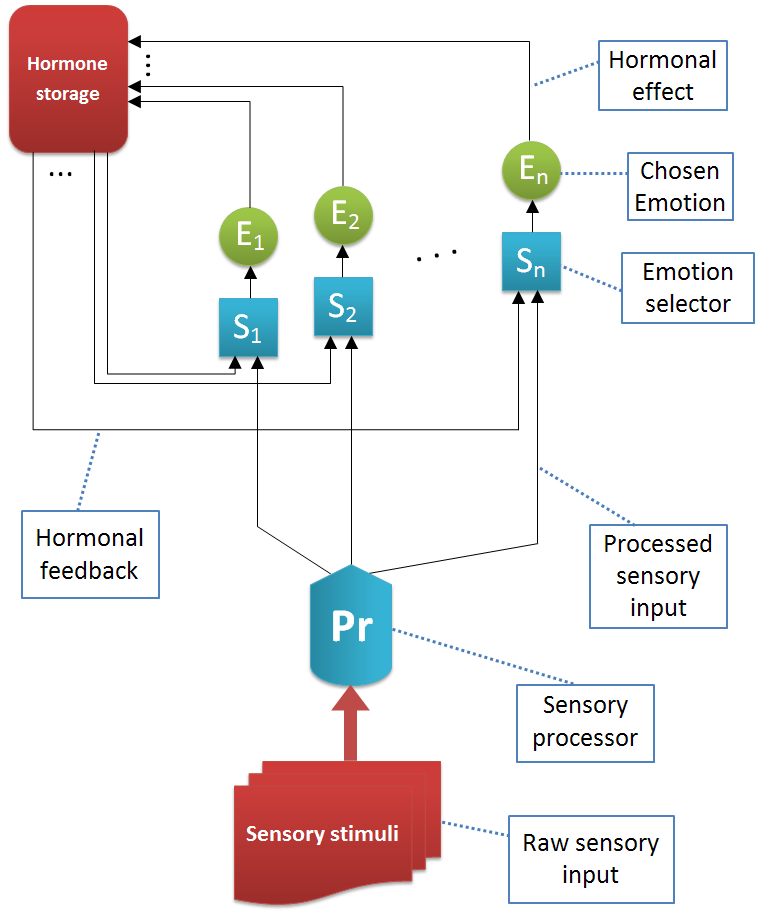
\includegraphics[width=400pt]{figs/affectiveSubsystem.png}
	\caption{Affective subsystem; specialisation of the global neural architecture. In plastic neural systems, selections may change over time.}
	\label{fig:affectiveSubsystem}
\end{figure}

\pagebreak
The main advantage of Gadanho's and Hallam's model is that (a) it is sufficiently generic to accommodate various schemas and (b) posits an internal state (the hormone storage), giving agents a certain inertia. For example, one can imagine integrating a many-dimensional model like Brazeal's \cite{breazeal2003} detailed taxonomy of emotion like Ortony's OCC model \cite{ortony1988}. The existence of an internal state is necessitated by the simply observation that our internal world is not solely dependent on momentary stimuli, but merely influenced by them. The idea of a hormone storage might be a simplistic approximation but it, too, can be refined as needed.\footnote{It might be tempting to simply replace the hormone storage with the message space, but doing so would ignore the role that neurotransmitters like dopamine and serotonin play in cognition, irrespective of the purely computational activity of brain components.} Figure~\ref{fig:sensoryPerception} shows the adapted model. The general structure was retained, but the set of sensations was replaced by the sensory processor described in Section~\ref{sec:sensoryPerception} and, instead of a single dominant emotion, competing emotions simply emit messages which are used by execute components and the world simulation.

\subsubsection{Affective subsystems}

In this section, I will develop the concept of ``emotion'' in greater detail. The process shown in Figure~\ref{fig:affectiveSubsystem} might suggest we simply have a collection of emotions and that all emotions are essentially equal, but I submit that this is not so. Instead, I propose the existence of various subsystems, each responsible for a group of emotions, and each with its own history and distinctive tasks. In the rest of this work, the following two assumptions will be made:

\begin{enumerate}
	\item {\em ``Emotion'' is not a singular phenomenon.} Specifically, this is contradicts many-dimensional models of emotions which propose one, two, three or four axes and a corresponding vector space in which every emotion is a point. Such a view implies that all emotions share a neurological template which is parametrized with coordinates to result in different experiences.
	\item {\em There exist emotions which are both different in kind and which pertain to different subsystems in the brain.} This implies that emotions cannot morally be seen as a homogeneous set $\{E_1,\dots,E_n\}$. Instead, a number of distinct subsystems are necessitated, each responsible for the causation and processing of a group of emotions. Given this, the only substantial aspect any two emotions might have in common would be our referring to both of them as ``emotion''.
\end{enumerate}

Both of these assumptions are rather concrete and thus deserve evidence. In 1999, Davidson and Irwin, using PET and fMRI scanning, found two different systems mediating approach- and avoidance related behaviors \cite[p. 13]{davidson1999}:

\begin{quote}
A large body of lesion, neuroimaging and electrophysiological data supports the view that the prefrontal cortex (PFC) is an important part of the circuitry that implements both positive and negative affect. ($\dots$)
A number of early studies that evaluated mood subsquent to brain damage suggested that patients with damage to the left hemisphere, particularly in PFC, were more likely to develop deppressive symptoms compared with patients having lesions in homologous regions of the right hemisphere. ($\dots$)
The general finding of left dorso-lateral PFC damage increasing the likelihood of deppressive symptoms has been interpreted to reflect the contribution of this cortical territory to certain features of positive affect, which, when disrupted, increases the probability of depressive symptomatology.
\end{quote}

In this, they echo earlies findings by Cacioppo et al. \cite{cacioppo1999}, Gray \cite{gray1994} and Lang et al. \cite{lang1990} that affect is lateralized, with different hemispheres being responsible for different categories of feeling. It therefore stands to reason that different emotions, being generated by different brain regions, should therefore also be different in their character.

Further, much research has been done in the area of so-called {\em basic emotions} --- a small set of emotions are acknowledged as being both elementary and characteristically distinct from each other. The Cambridge Handbook of Affective Neuroscience provides a good overview of the basic emotion theory \cite[pp. 9-10]{cambridgeAff}. Matsumoto and Eckman \cite{matsumoto2009}, for instance, identified seven basic emotions: happiness, surprise, contempt, sadness, fear, disgust, and anger.

Damasio \cite{damasio1998}, drawing upon neuroscientific findings, sketches a model of affect mainly involving the prefrontal cortex, but alos the amygdala, the hypothalamus, and the anterior cingulate cortex, as seen in Figure~\ref{fig:damasioSystem}.

\begin{figure}
	\centering
	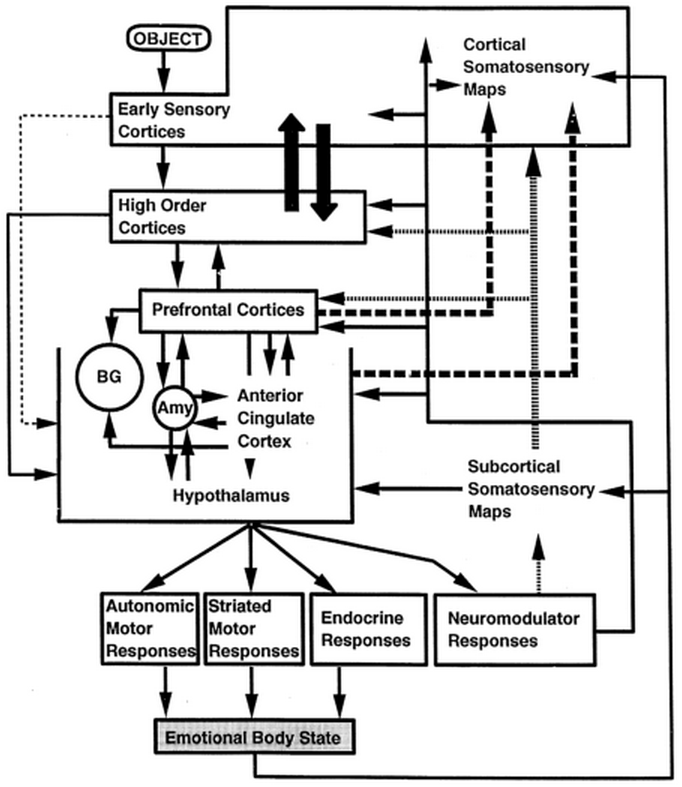
\includegraphics[width=250pt]{figs/damasioSystem.png}
	\caption{Neurological structure of affect, according to Damasio \cite{damasio1998}.}
	\label{fig:damasioSystem}
\end{figure}

In the same article, he describes how different brain regions are responsible for different kinds of emotion:

\begin{quotation}
	Equally problematic is the widespread view that the limbic system is the neural basis for all emotions. A rich body of evidence tells us that this is just not the case. Both within and around the limbic system, circuitry connection varied neural sites supports the operation of different emotion. For instance, work on aversive conditioning in rodents has shown that the amygdala is certainly involved in negative emotions such as fear [10,6]. {\em Work in humans, on the other hand, has not only confirmed the amygdala's involvement in negative emotions such as fear and anger, but also shown that the amygdala is not involved in the processing of positive emotions such as happiness, or negative emotions such as disgust.} [emphasis mine]
\end{quotation}

The last sentence of that quotation is especially revealing: it states that the neurological distinction is not simply one between positive and negative, or one between approach- or avoidance-related emotions, but that each emotion has its own profile of neurological activity and involves its own peculiar set of brain structures.

These facts make it quite clear that emotions are not simply homogeneous phenomena, being induced by a single system in the brain; rather, they are different in character and in the neural structures they involve. 

\paragraph{Structure of affect} The system depicted in Figure~\ref{fig:affectiveSubsystem} left several parts unspecified: the sensory processor $\Pr$, the emotion selectors $S_1,\dots,S_n$ and the messages sent by the chosen emotions into the message space. In the following paragraphs, I will flesh out that model in greater detail, building principally on the work of Sander, Grandjean and Scherer \cite{DBLP:journals/nn/SanderGS05}. Sander and colleagues partitioned the emotion process into four stages, as shown in Figure~\ref{fig:sanderSystem}. The first is {\em relevance}, which functions as a filter and detects the intrinsic pleasantness and the level of (emotional) attention that a stimulus demands. The processes of this stage, roughly speaking, correspond to the work of the sensory processor $\Pr$. The second stage is {\em implication}, where reasoning becomes engaged in order to determine the cause, likely outcome, and urgency of the perceived facts. At this stage, emotions like joy, anger, contentment, disgust, etc. are evoked, together with approach- and avoidance-related behaviours --- this corresponds to the emotion selectors $S_1,\dots,S_n$. Deliberate strategies come only in the next stage: {\em coping}. In it, reasoning and planning become fully engaged. The fourth stage is {\em normative significance} and deals, in essence, with moral concerns, both internal and those of other agents.

\begin{figure}
	\centering
	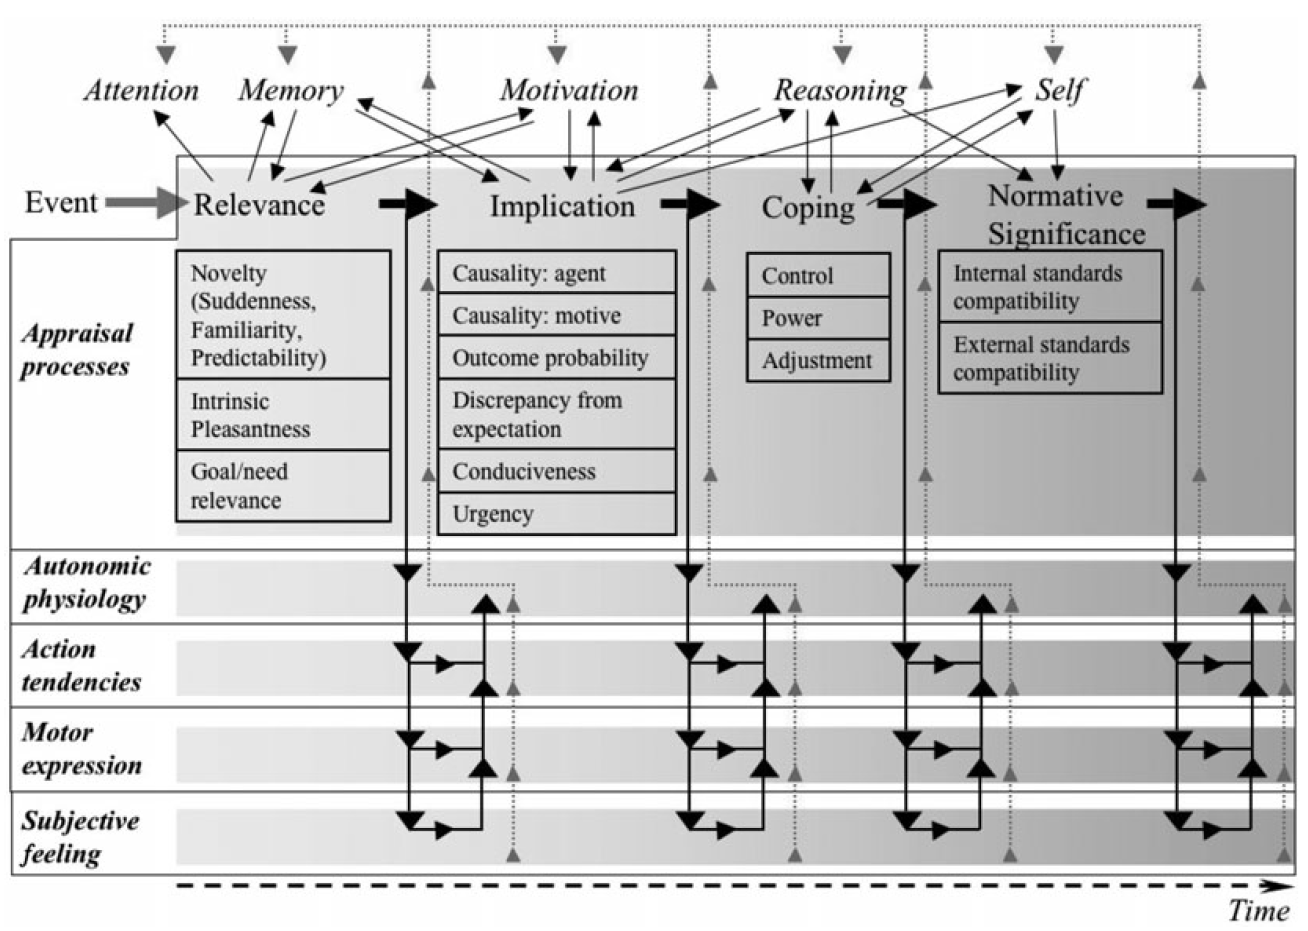
\includegraphics[width=440pt]{figs/sanderSystem.png}
	\caption{The four-stage emotion process according to Sander et al, consisting of relevance, implication, coping and normative significance.}
	\label{fig:sanderSystem}
\end{figure}

The system of Sander et al. presents the {\em vertical view} (the pipeline) of emotion; however, it does not describe the broader context into which this system is embedded. In particular, it does not address the interactions with perception, memory, and reasoning. Based on the evidence discussed above, I shall now present a {\em horizontal view} and construct a model of the hypothesized emotional subsystems and their interactions with other parts of the brain. Since no established vocabulary seems to exist in this specific are I shall first introduce a number of terms.

\begin{definition}[Evocative system]
An evocative system is a subsystem in the brain responsible for evoking consciously experienced affect within an agent based on internal or external stimuli.
\end{definition} 

I propose the existence following four evocative systems:

\begin{enumerate}
	\item \textbf{pre-social behavior control}, encompassing the kinds of mental states that we see in most large animals, such as fear, aggression, contentment and eagerness;
	\item \textbf{attention-refocusing}, primarily dealing with surprise;
	\item the \textbf{social judgement system}, which deals with our appraisal of agents in social settings and is responsible for feelings like disgust, contempts, respect and worship;
		\begin{enumerate}
				\item the \textbf{social reflective system}, which is part of the social judgement system and is responsible for exlusively self-reflective emotions like pride or shame;
				\item the \textbf{social normative system}, responsible for normative/moral judgements;
		\end{enumerate}
	\item the \textbf{aesthetic system}, which is concerned with aesthetics, but also influences complex experiences like mathematical intuition or musical taste.
\end{enumerate}

This list can be found in different forms in more extensive taxonomies, chiefly among them in Ortony's OCC model \cite{ortony1988}, although the taxonomies tend to neglect the evolutionary dimension and the chronology of these systems.

\begin{definition}[Executive system]
An executive system is a subsystem in the brain which regulates attention, makes decisions and causes deliberate motor action in an agent.
\end{definition}

Up to this point, the executive functions have not been discussed in detail, as they are not the focus of this work. Any description of affect, however, would be incomplete without them, as attentional and behavioural changes are the sole point of emotions. Very broadly speaking, we can divide executive functions into four categories:

\begin{enumerate}
	\item \textbf{sub-conscious motor control}: instinctive reaction, such as the jerking away from pain, jumping when startled, and turning towards interesting visual stimuli;
	\item \textbf{conscious motor control}: deliberate, planned action which the agent experiences as a choice;
	\item \textbf{sub-conscious mental control}: involuntary but consciously experienced changes to the mind-state of an agent which are perceived as activity rather than mere feeling. This includes like obsessing over an issue, manias, fantasies insofar as involuntary, etc.
	\item \textbf{conscious mental control}: deliberate mental changes of an agent. This includes the making of decisions, the deliberate focusing of attention, deliberate planning, deliberate strategy selection, and so forth.
\end{enumerate}

\paragraph{Pre-social behavior control} 

\paragraph{Social judgement system}

\paragraph{Social reflective system}

\paragraph{Aesthetic judgement system}

\section{Interaction between affect and world simulation}

Section~\ref{sec:worldSimulation} outlined what could be called {\em deliberate action} in the from of a planner-world-simulator loop. Section~\ref{sec:affect} described the structure and components of affect. These systems are of course not isolated from each other; emotional states influence both the planner's chosen heuristics and the world simulator's creation of worlds. In addition, attention, also influenced by affect, controls the allocation of cognitive resources. We now explore these relationships in further detail.

\paragraph{Planning as search} In the AI literature, search algorithms are of great importance. In this context, we can view the loop between planner and world simulator as a greedy search: the planner chooses the nodes which are to be expanded and sends them to the world simulator. It, in turn, performs the expansion by simulating the appropriate worlds. These simulated worlds are sent back to the planner for evaluation regarding desirability (i.e. cost). This presents an obvious problem: since greedy search is not complete, our planner-world-simulator loop can't be complete either. In fact, the situation is worse --- greedy search computes the cost of all candidates for expansion and chooses the cheapest, whereas our planner, being heuristic, might not consider certain nodes at all.

This might seem damning, but we must also consider the interaction with attention and memory. First, planned steps are committed to memory and thus, we gain access to past costs. An agent doesn't plan blindly, but can recall how long its plans are and what costs past planned steps entail. Given this information, we can turn the greedy algorithm into an A$^*$ search, with the qualification that the planner might not consider certain nodes. The mechanism of attention can further be used to enhance the search: if planning along a certain path takes too long, the agent might decide to abandon it altogether and start afresh with a different strategy. This failure too is stored in memory and can influence the planner in the new planning process by making the proposing of steps of the previously pursued path  unlikely.

\section{Implementation}

\subsection{World}

The choice of world profoundly affects the implementation of the agent --- its perception, knowledge base, and the range of performed actions. On one hand, it should be simple enough to permit a reasonably small and effective agent which does not get bogged down with irrelevant details; on the other, the world should be sufficiently complex to allow the agent to shine. This is especially true in the case of an affective agent whose actions should be visibly influenced in rich and subtle ways by its emotional state. For this evaluation, we choose a version of the Wumpus world --- a standard in AI, described in Russell and Norvig's {\em Artificial Intelligence: A Modern Approach} \cite{norvig}

\subsubsection{Wumpus world}







In this section, having sketched the underlying model and the relevant subsystems, I move on to the description of an implementation of an affective artificial agent. Its structure will necessarily be a gross simplification of any biological agent, but it will serve as a proof-of-concept.\\

\noindent
Note: instead of detailed partial descriptions, I, for now, sketch the rough outline of the proposed implementation to give a complete picture.

Outline of algorithm (provisional):

\begin{enumerate}
	\item One agent is composed of the following components:
		\begin{enumerate}
			\item Sensory perception
			\item Affect
			\item Planner and world simulator
			\item Memory
			\item Attention
		\end{enumerate}
	\item Sensory perception will be highly domain-dependent and, by necessity, simplified. Domains might be flatland or some custom-made game scenarios. In essence, it will deliver facts about objects and events in the world, bypassing the problem of faithfully implementing sight, hearing, smell, balance, pain, etc.
	\item At each step, sensory facts are put into the neural system's message space and are consumed by the evocative systems (PSBC, attention-refocusing, SJS, AS).
	\item The primitive parts of the PSBC can affect the executive system directly. Its higher-level parts, as well as the other three systems, work in the following way:
		\begin{enumerate}
			\item Attention-refocusing directs cognitive resources to stimuli it deems important. As a result, the priority of (certain) sensory messages is increased, increasing their influence on PSBC and the SJS.
			\item PSBC and the SJS evoke certain emotions. Thereby, they might set goals for the agent. This setting of goals engages the planner and world simulator, which try to devise a plan to meet said goal --- this is implemented via DLV-hex programs. These DLV-hex program, in turn, call the emotional systems in order to modulate both the planner and the world simulator according to the emotional state of the agent.
			\item Planned steps are committed to (short-term) memory.
		\end{enumerate}
	\item The PSBC's effects and the plans created by the agent are then translated into choices via conscious motor control, with the proviso that plans, even if deemed effective, are not executed under all circumstances: if some step is deemed too undesirable according to the emotional state of the agent at the time of execution, it might be abandoned and the planning stage starts anew. The kinds of actions that the agent executes are again highly dependent on the domain. Full physical simulation of a body would be prohibitively expensive, but simple, atomic actions like ``move left'' or ``attack'' would suffice for modelling purposes.
	\item The AS and sub-conscious motor control will not be implemented for the time being, as they are only relevant in highly sophisticated worlds.
\end{enumerate}

\pagebreak

\nocite{*}


\bibliographystyle{plain}
\bibliography{proposed_model}


\end{document}
